\begin{figure}
	\centering
	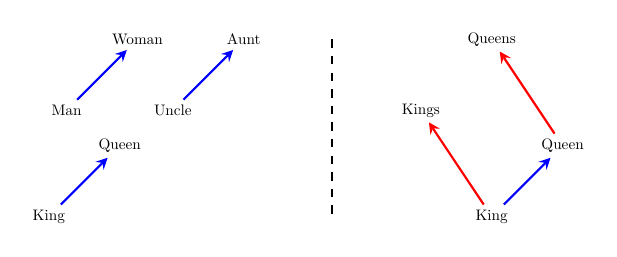
\begin{tikzpicture}[
		scale=0.45,
		every node/.style={scale=0.55},
		arr/.style={-stealth,thick}
	]

		\node (M) at (0,0) {Man};
		\node (W) at (2,2) {Woman};
		\draw[arr,blue] (M) -- (W);
		
		\node (U) at (3,0) {Uncle};
		\node (A) at (5,2) {Aunt};
		\draw[arr,blue] (U) -- (A);
		
		\node (K1) at (-0.5,-3) {King};
		\node (Q1) at (1.5,-1) {Queen};
		\draw[arr,blue] (K1) -- (Q1);

		\draw[dashed,thick] (7.5,2) -- (7.5,-3);


		\node (K2) at (12,-3) {King};
		\node (Ks) at (10,0) {Kings};
		\node (Q2) at (14,-1) {Queen};
		\node (Qs) at (12,2) {Queens};

		\draw[arr,red] (K2) -- (Ks);
		\draw[arr,red] (Q2) -- (Qs);
		\draw[arr,blue] (K2) -- (Q2);

	\end{tikzpicture}
\end{figure}